%%% LaTeX Template: Article/Thesis/etc. with colored headings and special fonts
%%%
%%% Source: http://www.howtotex.com/
% vim: set spell spelllang=es syntax=tex :

\documentclass[12pt]{article}
\usepackage{styles/apuntes-estilo}
\usepackage{styles/egyptian}
\usepackage{fancyhdr,lastpage}
\usepackage{hyperref}
\usepackage[inline]{enumitem}

\def\maketitle{

\makeatletter
{\color{bl} \centering \huge \sc \textbf{ Trabajo práctico N° 7\\ \large
\vspace*{-8pt} \color{black} Redes de computadoras \vspace*{8pt} }\par}
\makeatother

\makeatletter
% vim: set spell spelllang=es syntax=tex :
 {\centering \small 
    Introducción a la computación\\
    Departamento de Ingeniería de Computadoras \\
    Facultad de Informática - Universidad Nacional del Comahue \\
    \vspace{20pt} }
\makeatother

\vspace{-2.5cm}
\mbox{\hspace{-1cm}\includegraphics[width=3cm,height=3cm]{logos/uncoma.pdf}\hspace{12cm}
    
\includegraphics[width=3cm,height=3cm]{logos/fai.pdf}}



}

% Custom headers and footers
\fancyhf{} % clear all header and footer fields
\fancypagestyle{plain}{\fancyhf{}}
\pagestyle{fancy}
\lhead{\footnotesize TP N° 7 - Redes de computadoras}
\rhead{\footnotesize \thepage\ }

\def\ti#1#2{\texttt{#1} & #2 \\ }

\begin{document}

\thispagestyle{empty}
\maketitle
\setlength{\parindent}{1pt}

\textbf{Objetivo:} Comprender conceptos básicos referidos a una red de
computadoras.

\textbf{Bibliografía básica:}

\vspace{-2\topsep}
\begin{itemize}

    \itemsep2pt \parskip0pt \parsep0pt

    \item Presentación del tema y apunte de cátedra en Pedco.

    \item James F. Kurose, Keith W. Ross. Computer Networking: a top down
        approach. Sixth edition. Editorial Pearson Addison-Wesley, 2013.  ISBN
        978-0-13-285620-1.

    \item James F. Kurose, Keith W. Ross. Redes de computadoras: un enfoque
        descendente. Quinta edición. Editorial Pearson Addison-Wesley, 2010.
        ISBN 978-84-7829-119-9

\end{itemize}

\begin{enumerate}

    \item Explicar qué es una red de computadoras.

    \item Explicar la clasificación básica de las redes: \emph{LAN},
        \emph{MAN}, \emph{WAN}.

    \item Definir protocolo y explicar su utilidad.

    \item Describa qué es un paquete de red.

    \item ¿Cuál es el formato de las direcciones \emph{IPv4}? ¿Es cierto que
        cada nodo solo puede tener una única dirección \textbf{IP}?¿Es válida
        la dirección \emph{IPv4} 312.18.1.1? ¿Por qué?

    \item ¿Cuál es el objetivo del \emph{routing} (enrutamiento)? Explicar
        cómo se lleva a cabo.

    \item Las máscaras de red permiten agrupar direcciones en las tablas de
        enrutamiento, ¿por qué interesa agrupar direcciones?

    \item Respecto a los nombres de dominio:

    \begin{enumerate}

        \item Explicar su utilidad

        \item ¿Cómo hace un navegador en un host para conocer qué dirección de
            red tiene \url{www.afa.com.ar}? Además, para este ejemplo,
            explicar quién gestiona cada uno de los servidores de nombres de
            dominio.

    \end{enumerate}

\end{enumerate}

\subsection*{Enlaces}

\textbf{Nota:} considere la velocidad de la luz como $300000 km/s$.

\begin{enumerate}

    \item Qué tiempo de propagación tendrá un enlace de fibra óptica de $1500
        km$?

    \item El satélite \textbf{ARSAT} se encuentra aproximadamente a $36000 km$
        de la Tierra ¿Cuál es el tiempo de propagación de una señal enviada
        del satélite a la Tierra? 

    \item Cuál es el tiempo de transmisión de un bit usando un enlace de $3
        Mb/s$? ¿Y el de un byte? ¿Y el de un archivo de $10 kB$ de datos? 

    \item Dado un archivo de $38 MB$, ¿cuánto tiempo cuesta descargar este
        archivo por un canal de $56kb/s$? ¿Y por uno de $1Mb/s$? 

    \item En cuánto tiempo se transferirán completamente $10 kB$ de datos, por
        un enlace con un tiempo de transmisión de $0.3 µs/b$ y un tiempo de
        propagación de $100 ms$? 

    \item Una cámara en la base lunar toma fotos de la Tierra y las graba en
        formato digital. Suponga que una misión de control en la Tierra desea
        descargar la imagen más reciente, que es de $25 MB$, usando un enlace
        con un tiempo de transmisión de $100 Mb/s$. ¿En cuánto tiempo se
        transferirá completamente la imagen desde la luna? La distancia de la
        Luna a la Tierra es aproximadamente $325000 Km$ y los datos viajan a
        la velocidad de la luz.
        
    \item ¿Qué velocidad de transmisión debe tener un enlace con tiempo de
        propagación de $120 ms$ para que $10 kB$ lleguen al otro extremo del
        enlace en $125 ms$?

\end{enumerate}

\subsection*{Protocolo}

Los protocolos definen las reglas básicas por las cuales dos entidades se
comunican. Un protocolo consta de "mensajes" entre las partes, y a través de
una secuencia determinada de dichos mensajes se logra una correcta
comunicación entre ellas.

\begin{enumerate}

    \item A continuación se define un protocolo de comunicación hipotético
        entre dos personas, para que una de ellas (el proveedor) otorgue
        cierta información a la otra (consumidor). Los mensajes \textbf{no
        están ordenados en la lista, simplemente se mencionan los mensajes
        disponibles}.

        \begin{tabular}{|l|l|}
            \hline
            \textbf{Mensajes del proveedor} & \textbf{Mensajes del
            consumidor}\\
            \hline
            ``Hola ¿quién sos?" & ``Hola.''\\
            ``¿Qué necesitas?'' & ``Mi nombre es \$NOMBRE.''\\
            ``La fecha de hoy es \$FECHA.'' & ``La fecha de hoy.''\\
            ``\$X metros son \$Y centímetros." & ``Convertir \$X metros a
            centímetros.''\\
            & ``¡Eso es todo!''\\
            \hline
        \end{tabular}

        En este protocolo, el consumidor es quien inicia la comunicación, con
        el mensaje ``Hola''. Observe además, que se ha usado el símbolo ``\$''
        para indicar que esa parte del mensaje puede cambiar en función del
        mensaje en particular. Por ejemplo, un mensaje concreto de ``Convertir
        \$X metros a centímetros'' sería ``Convertir 10 metros a
        centímetros''.

    \begin{enumerate}

        \item La siguiente secuencia de mensajes entre un proveedor y un
            consumidor está desordenada, ordene dichos mensajes de la forma
            natural que ocurrirían al usar este protocolo: 

        \begin{itemize}

            \item La fecha de hoy es 8 de febrero del 1996.

            \item ¡Eso es todo!

            \item La fecha de hoy.

            \item ¿Qué necesitas?

            \item Hola ¿quién sos?

            \item Mi nombre es Juan.

            \item ¿Qué necesitas?

            \item Hola.

        \end{itemize}

        \item Extienda el conjunto de mensajes del protocolo para que el
consumidor pueda consultar al proveedor la temperatura actual.

    \end{enumerate}

    \item La World Wide Web se apoya en el protocolo \emph{Hyper Text
        Transport Protocol} para que los navegadores web se comuniquen con los
        servidores y obtengan contenido desde ellos. Cuando se ingresa una
        dirección en el navegador se intercambian una serie de mensajes
        \emph{HTTP} hasta lograr que el servidor envíe la información
        solicitada al cliente. 

    \begin{enumerate}

    \item Abra una terminal de texto en cualquier sistema Linux (o Windows que
        disponga del comando telnet), y ejecute el siguiente comando (respete
            las minúsculas): 

            \begin{verbatim}
$ telnet www.uncoma.edu.ar 80
            \end{verbatim}

            Este comando no es parte del protocolo \emph{HTTP}, solamente
            abrirá una conexión entre el programa \textbf{telnet} y el
            servidor Web de \emph{UNCOMA}. Una vez establecida la conexión, se
            pueden intercambiar mensajes entre las partes (cliente y
            servidor).

    \item A continuación pruebe los siguientes mensajes (luego de cada
        mensaje, la conexión se cerrará, por lo que deberá volver a ingresar
            la orden \textbf{telnet www.uncoma.edu.ar 80}) y explique
            brevemente con sus palabras la respuesta que recibe. Utilice la
            siguiente \emph{URL} para comprender las respuestas del protocolo
            \emph{HTTP} del servidor de \emph{UNCOMA}:
            \textbf{https://es.wikipedia.org/wiki/Anexo:C\'odigos\_de\_estado\_HTTP}

            Luego de cada mensaje presione enter dos veces. Debe volver a
            ejecutar el comando telnet luego de cada respuesta.

        \begin{enumerate}
                
            \item HOLA

            \item \emph{(no presionar nada, esperar aproximadamente 1 minuto)}

            \item GET / HTTP/1.0

            \item GET /noexiste HTTP/1.0

        \end{enumerate}

    \end{enumerate}

    \item Uno de los protocolos más útiles para los usuarios y utilizado
        diariamente por prácticamente toda la Internet es el \emph{Domain Name
        System} (DNS, Sistema de nombres de dominio). Este protocolo permite
        convertir nombres legibles por usuarios (Ej: \url{www.wikipedia.org})
        en números \emph{IP} que corresponden a direcciones de computadoras en
        Internet.

        En el ejercicio anterior, al usar el comando \textbf{telnet
        www.uncoma.edu.ar 80}, lo primero que hace el programa telnet antes de
        establecer la conexión es convertir \url{www.uncoma.edu.ar} en el
        número 170.210.81.106 haciendo uso del protocolo \emph{DNS}, y luego
        conociendo este número es cuando puede establecer la conexión.

        \begin{enumerate}

            \item Utilice el comando "ping", que envía un pequeño paquete de
                información hasta un destino y espera una respuesta igual,
                para conocer las direcciones correspondientes a los siguientes
                servidores: 

            \begin{itemize}

                \item \url{www.wikipedia.com}

                \item \url{www.google.com.ar}

            \end{itemize}

                \textbf{Nota:} como alternativa al comando "ping", se puede utilizar el
                comando "host".
            
            \item Explique con sus palabras los beneficios de utilizar nombres
                en vez de números para los usuarios ¿Y para las máquinas?

        \end{enumerate}

\end{enumerate}

\subsection*{Direcciones}

\begin{enumerate}

    \item Un sistema recibe la siguiente dirección \textbf{1100 0000 1010 1000
        0000 0000 0000 0001}(32 bits en total). Exprese la dirección en
        notación decimal punteada. 

    \item Exprese las siguientes direcciones binarias en notación decimal
        punteada: 

    \begin{enumerate}

        \item 0000 1010 0000 0001 0100 0101 1010 0111

        \item 1100 1000 0011 0001 1111 1111 0111 1101

        \item 0100 0000 1110 1001 1011 1010 0101 1110

    \end{enumerate}

    \item Una organización recibe la dirección 130.21.0.0, con un prefijo cuya
        longitud es de 16 bits. Indique el rango de direcciones que puede
        utilizarse. 

%    \item Para las siguientes direcciones de red, calcule el rango de posibles
%        direcciones, expresándolas en notación decimal con puntos.
%
%    \begin{enumerate}
%
%        \item 192.56.0.0 con prefijo de 24 bits.
%
%        \item 134.142.0.0 con prefijo de 16 bits.
%
%        \item 120.0.0.0 con prefijo de 8 bits.
%
%    \end{enumerate}
%
%    \item Dado el rango de direcciones 168.45.0.0 a 168.45.255.255 indique
%        cuántos bits tiene el prefijo utilizado. Luego escriba la máscara
%        correspondiente en formato binario y en formato decimal con puntos. 
%
%    \item Dados los siguientes rangos de direcciones, indique la longitud del
%        prefijo y escriba la máscara correspondiente en notación decimal con
%        puntos.
%
%    \begin{enumerate}
%
%        \item 170.140.0.0 a 170.140.127.255 
%
%        \item 193.126.128.0 a 193.126.128.255 
%
%        \item 193.220.1.192 a 193.220.1.255
%
%    \end{enumerate}
%
\end{enumerate}

\subsection*{Enrutamiento}

Considerando el siguiente diagrama de una red de dispositivos donde \emph{R1},
\emph{R2}, \emph{R3}, \emph{R4} y \emph{R5} son routers, y \emph{A}, \emph{B},
\emph{C}, \emph{D} y \emph{E} son \emph{host}:

    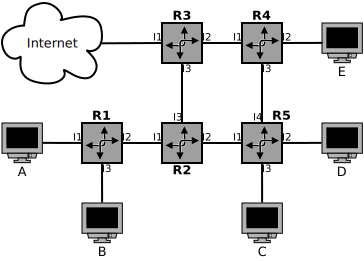
\includegraphics[width=0.50\textwidth]{img/red01.pdf}

Donde las tablas de enrutamiento de los routers son las siguientes:

\textbf{Router R1}

\begin{tabular}{|c|c|c|}
    \hline
    Destino & Máscara & Interfaz \\
    \hline
    10.0.0.224 & 255.255.255.240 & I1 \\
    \hline
    10.0.0.240 & 255.255.255.240 & I3 \\
    \hline
    0.0.0.0 & 0.0.0.0 & I2 \\
    \hline
\end{tabular}

\textbf{Router R2}

\begin{tabular}{|c|c|c|}
    \hline
    Destino & Máscara & Interfaz \\
    \hline
    10.0.0.182 & 255.255.255.254 & I2 \\
    \hline
    10.0.0.224 & 255.255.255.224 & I1 \\
    \hline
    0.0.0.0 & 0.0.0.0 & I3 \\
    \hline
\end{tabular}

\textbf{Router R3}

\begin{tabular}{|c|c|c|}
    \hline
    Destino & Máscara & Interfaz \\
    \hline
    10.0.0.180 & 255.255.255.252 & I2 \\
    \hline
    10.0.0.224 & 255.255.255.224 & I3 \\
    \hline
    0.0.0.0 & 0.0.0.0 & I1 \\
    \hline
\end{tabular}

\textbf{Router R4}

\begin{tabular}{|c|c|c|}
    \hline
    Destino & Máscara & Interfaz \\
    \hline
    10.0.0.180 & 255.255.255.254 & I2 \\
    \hline
    10.0.0.182 & 255.255.255.254 & I3 \\
    \hline
    0.0.0.0 & 0.0.0.0 & I1 \\
    \hline
\end{tabular}

\textbf{Router R4}

\begin{tabular}{|c|c|c|}
    \hline
    Destino & Máscara & Interfaz \\
    \hline
    10.0.0.183 & 255.255.255.255 & I2 \\
    \hline
    10.0.0.182 & 255.255.255.255 & I3 \\
    \hline
    0.0.0.0 & 0.0.0.0 & I1 \\
    \hline
\end{tabular}

\begin{enumerate}

    \item ¿Por qué routers pasará un paquete que tenga como origen el
        \emph{host A} y destino el \emph{host} con número de \emph{IP
        10.0.0.181}?

    \item ¿Por qué routers pasará un paquete que tenga como origen el
        \emph{host E} y destino el \emph{host} con número de \emph{IP
        10.0.0.225}?

    \item ¿Por qué routers pasará un paquete que tenga como origen el
        \emph{host C} y destino el \emph{host} con número de \emph{IP
        192.168.0.1}?

    \item ¿Puede determinar la \emph{IP} del \emph{host A}?

    \item ¿Puede determinar la \emph{IP} del \emph{host C}?

\end{enumerate}

\end{document}
